\documentclass[border=15pt]{standalone}
\usepackage{tikz,amsmath}
\usetikzlibrary{arrows.meta,decorations.pathreplacing}

% ========== 配色方案 ==========
\definecolor{inFill}{RGB}{183,224,177}       % 输入特征图绿色
\definecolor{inLine}{RGB}{32,102,32}
\definecolor{padFill}{RGB}{228,244,226}     % Padding 浅浅绿
\definecolor{padLine}{RGB}{120,170,120}     % Padding 边框柔和草绿

\definecolor{hidFill}{RGB}{199,203,243}     % 卷积核紫色
\definecolor{hidLine}{RGB}{52,58,143}

\definecolor{orFill}{RGB}{250,224,180}      % 中间特征图橙色 (Intermediate)
\definecolor{orLine}{RGB}{190,110,20}

\definecolor{outFill}{RGB}{243,199,199}     % 最终输出特征图红色
\definecolor{outLine}{RGB}{143,52,52}

\begin{document}
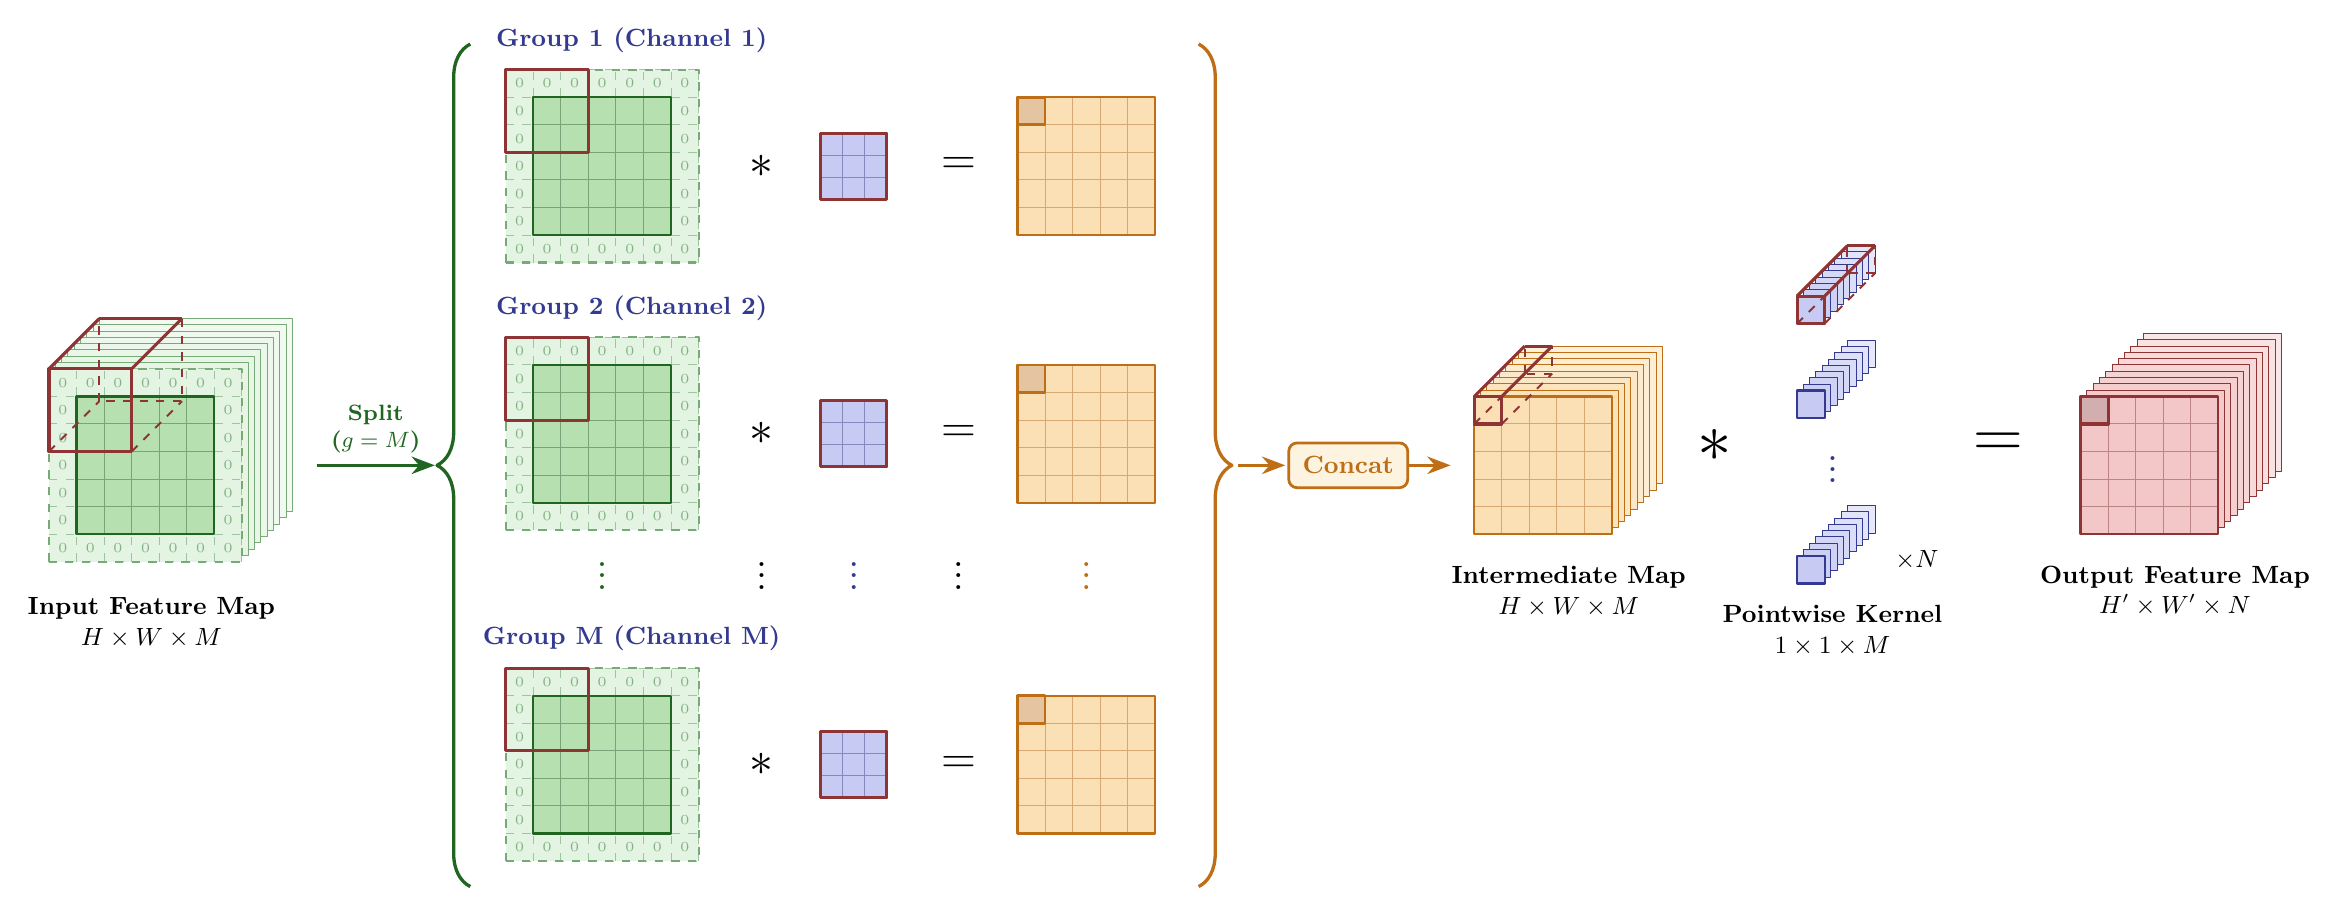
\begin{tikzpicture}[
    font=\small, line join=round,
    every node/.style={inner sep=0pt, outer sep=0pt, align=center}
  ]

  % ========== 基础二维单层特征图宏 ==========
  % #1: x, #2: y, #3: 网格边长格数, #4: 单格尺寸, #5: 颜色前缀
  \newcommand{\gridbox}[5]{%
    \fill[#5Fill] (#1,#2) rectangle ++(#3*#4, #3*#4);
    \draw[step=#4, #5Line!60, line width=.35pt, shift={(#1,#2)}] (0,0) grid (#3*#4, #3*#4);
    \draw[#5Line, thick] (#1,#2) rectangle ++(#3*#4, #3*#4);
  }

  % ========== 带 Padding 的二维单层切片宏 ==========
  % #1: x, #2: y, #3: 内层真实数据格数, #4: 每格尺寸, #5: 颜色前缀, #6: padding圈数
  \newcommand{\slicepad}[6]{%
    \pgfmathtruncatemacro{\totgrid}{#3 + 2*#6}
    \pgfmathsetmacro{\totdim}{\totgrid * #4}
    \pgfmathsetmacro{\indim}{#3 * #4}
    \pgfmathsetmacro{\padoff}{#6 * #4}
    % 1. Padding 填充与虚线网格
    \fill[padFill] (#1,#2) rectangle ++(\totdim,\totdim);
    \draw[step=#4, padLine!70, dashed, line width=.35pt, shift={(#1,#2)}] (0,0) grid (\totdim,\totdim);
    % 2. 真实数据填充与实线网格
    \fill[#5Fill] ({#1+\padoff},{#2+\padoff}) rectangle ++(\indim,\indim);
    \draw[step=#4, #5Line!60, line width=.35pt, shift={({#1+\padoff},{#2+\padoff})}] (0,0) grid (\indim,\indim);
    % 3. 边框
    \draw[#5Line, thick] ({#1+\padoff},{#2+\padoff}) rectangle ++(\indim,\indim);
    \draw[padLine, thick, dashed] (#1,#2) rectangle ++(\totdim,\totdim);
    % 4. 填充 0
    \pgfmathtruncatemacro{\lastidx}{\totgrid-1}
    \foreach \ix in {0,...,\lastidx}{%
      \node[font=\fontsize{5}{6}\selectfont, text=padLine!90] at ({#1+(\ix+0.5)*#4}, {#2+0.5*#4}) {0};
      \node[font=\fontsize{5}{6}\selectfont, text=padLine!90] at ({#1+(\ix+0.5)*#4}, {#2+(\lastidx+0.5)*#4}) {0};
    }
    \pgfmathtruncatemacro{\midend}{\lastidx-1}
    \foreach \iy in {1,...,\midend}{%
      \node[font=\fontsize{5}{6}\selectfont, text=padLine!90] at ({#1+0.5*#4}, {#2+(\iy+0.5)*#4}) {0};
      \node[font=\fontsize{5}{6}\selectfont, text=padLine!90] at ({#1+(\lastidx+0.5)*#4}, {#2+(\iy+0.5)*#4}) {0};
    }
  }

  % ========== 通用 3D 堆叠切片宏 ==========
  % #1: x, #2: y, #3: 网格格数, #4: 单元格尺寸, #5: 颜色前缀, #6: 叠加层数, #7: 层间深度步长
  \newcommand{\stackbox}[7]{%
    \foreach \k in {#6,...,1}{%
      \pgfmathtruncatemacro{\op}{round(100 - (55 * \k / #6))}%
      \fill[#5Fill!\op, draw=#5Line, line width=.35pt]
            ({#1+#7*\k},{#2+#7*\k}) rectangle ++(#3*#4,#3*#4);
    }
    \fill[#5Fill] (#1,#2) rectangle ++(#3*#4,#3*#4);
    \draw[step=#4, #5Line!60, line width=.35pt, shift={(#1,#2)}] (0,0) grid (#3*#4,#3*#4);
    \draw[#5Line, thick] (#1,#2) rectangle ++(#3*#4,#3*#4);
  }

  % ========== 带 Padding 的 3D 堆叠切片宏 ==========
  \newcommand{\stackboxpad}[8]{%
    \pgfmathtruncatemacro{\totgrid}{#3 + 2*#8}
    \pgfmathsetmacro{\totdim}{\totgrid * #4}
    \pgfmathsetmacro{\indim}{#3 * #4}
    \pgfmathsetmacro{\padoff}{#8 * #4}
    \foreach \k in {#6,...,1}{%
      \pgfmathtruncatemacro{\op}{round(100 - (55 * \k / #6))}%
      \fill[padFill!\op, draw=padLine, line width=.35pt]
            ({#1+#7*\k},{#2+#7*\k}) rectangle ++(\totdim,\totdim);
      \fill[#5Fill!\op, draw=#5Line, line width=.35pt]
            ({#1+#7*\k+\padoff},{#2+#7*\k+\padoff}) rectangle ++(\indim,\indim);
    }
    \fill[padFill] (#1,#2) rectangle ++(\totdim,\totdim);
    \draw[step=#4, padLine!70, dashed, line width=.35pt, shift={(#1,#2)}] (0,0) grid (\totdim,\totdim);
    \fill[#5Fill] ({#1+\padoff},{#2+\padoff}) rectangle ++(\indim,\indim);
    \draw[step=#4, #5Line!60, line width=.35pt, shift={({#1+\padoff},{#2+\padoff})}] (0,0) grid (\indim,\indim);
    \draw[#5Line, thick] ({#1+\padoff},{#2+\padoff}) rectangle ++(\indim,\indim);
    \draw[padLine, thick, dashed] (#1,#2) rectangle ++(\totdim,\totdim);
    \pgfmathtruncatemacro{\lastidx}{\totgrid-1}
    \foreach \ix in {0,...,\lastidx}{%
      \node[font=\fontsize{5}{6}\selectfont, text=padLine!90] at ({#1+(\ix+0.5)*#4}, {#2+0.5*#4}) {0};
      \node[font=\fontsize{5}{6}\selectfont, text=padLine!90] at ({#1+(\ix+0.5)*#4}, {#2+(\lastidx+0.5)*#4}) {0};
    }
    \pgfmathtruncatemacro{\midend}{\lastidx-1}
    \foreach \iy in {1,...,\midend}{%
      \node[font=\fontsize{5}{6}\selectfont, text=padLine!90] at ({#1+0.5*#4}, {#2+(\iy+0.5)*#4}) {0};
      \node[font=\fontsize{5}{6}\selectfont, text=padLine!90] at ({#1+(\lastidx+0.5)*#4}, {#2+(\iy+0.5)*#4}) {0};
    }
  }

  % ========== 1x1xM 立体卷积核宏 ==========
  % #1: x, #2: y, #3: 尺寸, #4: 叠加层数, #5: 步长
  \newcommand{\pwkernel}[5]{%
    \foreach \k in {#4,...,1}{%
      \pgfmathtruncatemacro{\op}{round(100 - (55 * \k / #4))}%
      \fill[hidFill!\op] ({#1+#5*\k},{#2+#5*\k}) rectangle ++(#3,#3);
      \draw[hidLine, line width=.35pt] ({#1+#5*\k},{#2+#5*\k}) rectangle ++(#3,#3);
    }
    \fill[hidFill] (#1,#2) rectangle ++(#3,#3);
    \draw[hidLine, thick] (#1,#2) rectangle ++(#3,#3);
  }

  % ========== 红色 3D 感受野/立体包裹框宏 ==========
  \newcommand{\prism}[5]{%
    \draw[outLine, dashed, line width=.7pt]
          (#1+#5,#2+#5) rectangle (#1+#5+#3,#2+#5+#4);
    \draw[outLine, line width=1.1pt]
          (#1+#5,#2+#5+#4) -- (#1+#5+#3,#2+#5+#4);
    \draw[outLine, dashed, line width=.7pt]
          (#1,#2)--(#1+#5,#2+#5) (#1+#3,#2)--(#1+#3+#5,#2+#5);
    \draw[outLine, line width=1.1pt] (#1,#2) rectangle (#1+#3,#2+#4);
    \draw[outLine, line width=1.1pt]
          (#1,#2+#4)--(#1+#5,#2+#5+#4) (#1+#3,#2+#4)--(#1+#3+#5,#2+#5+#4);
  }

  % =========================================================================
  % 【阶段一：Depthwise 卷积 (逐通道独立卷积)】
  % =========================================================================

  % 1. 左侧：总输入特征图 (5x5xM，加 Padding 后为 7x7xM，绿色)
  \stackboxpad{-5.4}{-1.225}{5}{0.35}{in}{8}{0.08}{1}
  \prism{-5.4}{0.175}{1.05}{1.05}{0.64}
  \node[align=center] at (-4.1, -2.0) {\textbf{Input Feature Map}\\$H\times W\times M$};

  % Split 箭头与文字 (通道拆分: g = M)
  \draw[->, >=Stealth, line width=1.2pt, inLine] (-2.0, 0) -- (-0.5, 0);
  \node[above, font=\bfseries\footnotesize, inLine] at (-1.25, 0.16) {Split\\($g=M$)};

  % 2. 左侧大花括号（包裹 M 个逐通道分支）
  \draw[inLine, line width=1.2pt, decorate, decoration={brace, amplitude=12pt}]
       (-0.05, -5.35) -- (-0.05, 5.35);

  % 3. 中间 Depthwise 卷积分支 (Group 1, Group 2, ..., Group M)
  \foreach \Y/\grp/\chn in {3.8/1/1, 0.4/2/2, -3.8/M/M}{
    \node[font=\bfseries\small, hidLine] at (2.0, \Y + 1.6) {Group \grp\ (Channel \chn)};

    % (1) 单通道输入切片 (7x7 带 padding)
    \slicepad{0.4}{\Y - 1.225}{5}{0.35}{in}{1}
    \draw[outLine, line width=1.1pt] (0.4, \Y + 0.175) rectangle ++(1.05, 1.05);

    % (2) 卷积乘号 *
    \node[font=\LARGE] at (3.65, \Y) {$\ast$};

    % (3) 独立单通道卷积核 (3x3，紫色)
    \gridbox{4.4}{\Y - 0.42}{3}{0.28}{hid}
    \draw[outLine, line width=1.1pt] (4.4, \Y - 0.42) rectangle ++(0.84, 0.84);

    % (4) 等号 =
    \node[font=\LARGE] at (6.15, \Y) {$=$};

    % (5) 单通道输出切片 (5x5，中间结果采用橙色)
    \gridbox{6.9}{\Y - 0.875}{5}{0.35}{or}
    \fill[orLine!40] (6.9, \Y + 0.525) rectangle ++(0.35, 0.35);
    \draw[orLine, line width=1pt] (6.9, \Y + 0.525) rectangle ++(0.35, 0.35);
  }

  % 纵向省略号
  \node[font=\LARGE, inLine]  at (1.625, -1.3) {$\vdots$};
  \node[font=\LARGE]          at (3.65,  -1.3) {$\vdots$};
  \node[font=\LARGE, hidLine] at (4.82,  -1.3) {$\vdots$};
  \node[font=\LARGE]          at (6.15,  -1.3) {$\vdots$};
  \node[font=\LARGE, orLine]   at (7.775, -1.3) {$\vdots$};

  % 4. 右侧大花括号与 Concat 拼接模块 (统一橙色)
  \draw[orLine, line width=1.2pt, decorate, decoration={brace, amplitude=12pt}]
       (9.2, 5.35) -- (9.2, -5.35);

  \draw[->, >=Stealth, line width=1.2pt, orLine] (9.7, 0) -- (10.3, 0);

  \node[draw=orLine, fill=orFill!40, rounded corners=3pt, line width=1pt,
        inner sep=5pt, font=\bfseries\small, text=orLine] (concat) at (11.1, 0) {Concat};

  \draw[->, >=Stealth, line width=1.2pt, orLine] (concat.east) -- (12.4, 0);

  % =========================================================================
  % 【阶段二：Pointwise 卷积 (逐点 1x1 跨通道卷积)】
  % =========================================================================

  % 5. Pointwise 输入：DW 卷积拼接后的中间特征图 (5x5xM，橙色)
  \stackbox{12.7}{-0.875}{5}{0.35}{or}{8}{0.08}
  % 红色立体虚线框覆盖贯穿所有 M 通道的 1x1xM 输入柱体
  \prism{12.7}{0.525}{0.35}{0.35}{0.64}
  \node[align=center] at (13.9, -1.6) {\textbf{Intermediate Map}\\$H\times W\times M$};

  % 卷积乘号 * (居中对齐于 Y = 0.25)
  \node[font=\Huge] at (15.75, 0.25) {$\ast$};

  % 6. Pointwise 卷积核 (展示三个 1x1xM 立体核，紫色)
  % 核 3 (最下方)
  \pwkernel{16.8}{-1.5}{0.35}{8}{0.08}

  % 核 2 (中间偏上)
  \pwkernel{16.8}{0.6}{0.35}{8}{0.08}

  % 核 1 (最上方，带红色立体选框)
  \pwkernel{16.8}{1.8}{0.35}{8}{0.08}
  \prism{16.8}{1.8}{0.35}{0.35}{0.64}

  % 中间省略号与数量标注 x N (位于核 2 与核 3 之间)
  \node[font=\LARGE, hidLine] at (17.25, 0.05) {$\vdots$};
  \node[font=\small, anchor=west] at (18.05, -1.2) {$\times N$};

  % 卷积核底部标签
  \node[align=center] at (17.25, -2.1) {\textbf{Pointwise Kernel}\\$1\times 1\times M$};

  % 等号 = (居中对齐于 Y = 0.25)
  \node[font=\Huge] at (19.35, 0.25) {$=$};

  % 7. 最终输出特征图 (5x5xN，红色)
  \stackbox{20.4}{-0.875}{5}{0.35}{out}{10}{0.08}
  % 左上角高亮单个映射输出像素点 (与核 1 和输入柱体完全水平对应)
  \fill[outLine!40] (20.4, 0.525) rectangle ++(0.35, 0.35);
  \draw[outLine, line width=1.1pt] (20.4, 0.525) rectangle ++(0.35, 0.35);
  \node[align=center] at (21.6, -1.6) {\textbf{Output Feature Map}\\$H'\times W'\times N$};

\end{tikzpicture}
\end{document}